% Chapter 5

\chapter{Results} % Main chapter title

\label{results} % For referencing the chapter elsewhere, use \ref{Chapter1} 

\lhead{Chapter 5. \emph{Results and Discussion}} % This is for the header on each page - perhaps a shortened title

%----------------------------------------------------------------------------------------

\section{Drag and lift on a cylinder}
The effect of the implemented algorithm in Nek5000 explained in Chapter~\ref{implementation} is
illustrated by solving a laminar flow test problem. 
The solution is compared with previously benchmark computations performed by a number of 
contributors~\cite{benchmark}. The test problem considered is steady flow with Re=20 in 
a rectangular channel past a cylinder. The drag and lift coefficients on the cylinder 
are calculated and compared to a pair of reference values. The results can be found in 
table~\ref{tab:testcase}. As the results clearly show the treatment of the geometry is 
crucial, both coefficients are computed with significantly better accuracy. 
%
\begin{table}
\centering
\begin{tabular}{l l c c c c}
		\toprule
		\# of Cells & Software & $c_D$ & $c_L$ & \%\textbf{Err} $c_D$ &\%\textbf{Err} $c_L$ \\ \midrule 
		2070 & Nek5000 (mid) & 6.18349 & 0.008939 & 0.030 & 4.19 \\ 
		2070 & Nek5000 (arc) & 6.18498 & 0.009413 & 0.006 & 0.13 \\
		3145728 & CFX 		 & 6.18287 & 0.009387 & 0.04 &0.15 \\
		3145728 & OF	     & 6.18931 & 0.00973 & 0.06 &3.5 \\
		3145728 & FEATFLOW   & 6.18465 & 0.009397 & 0.01 &0.05 \\
		\bottomrule	
	\end{tabular}
	\caption{Results for the drag and lift coefficients with reference values 
	$c_D = 6.18533$ and $c_L = 0.009401$.}
\label{tab:testcase}
\end{table}
%
The polynomial degree used in the calculations with Nek5000 was chosen as $p = 11 $ 
in all directions. The explicit number of cells is therefore $2070\cdot11^{3} = 2755170$,
approximately $88\%$ of the number of cells used for the benchmark simulations. Compared 
with the results from the other softwares applied in~\cite{benchmark} Nek5000 performs 
just as well or better in most cases. It should be mentioned that the division of the grid is done 
differently for Nek5000 so the comparison is not as direct as it may seem from the table.

\colorbox{yellow}{add more info about the mesh for this case??}

\subsection{Parameter adjustments in Nek5000}
As discussed in chapter~\ref{nek} there are many adjustments available in Nek. 
In order to enlighten the actual effect on the results, several different settings have 
been investigated and the results are presented. All simulations are performed as 
transient flows and the data collected in table~\ref{tab:perf} are gathered when the 
flow has reached a steady state solution. 

\colorbox{green}{Perform the different tests and show the difference.}

\begin{table}[h]
    \centering
    \begin{tabular}{c | c c c | c c | c c c}

         & \multicolumn{3}{|c|}{Settings} & \multicolumn{2}{|c|}{\% Error} & \multicolumn{3}{|c}{Data} \\\hline
         \#  & Aliasing & IOFS & Filter & $c_D$ & $c_L$ 
         & DT & CFL & T/Tstep \\ \hline 
         1 & No & No & No & 1.0 & 2.3 & 1e-04 & 2.03 & 2.1e-02 \\
    \end{tabular}
    \caption{Performance data for different settings in Nek5000}
    \label{tab:perf}
\end{table}
%----------------------------------------------------------------------------------------
\section{Gas dispersion in a simplified urban area} 
This case is a part of a larger project designed to evaluate different solvers 
ability to perform simulations of gas dispersion. An initial attempt to simulate the 
dispersion of gas was performed in Nek5000 with fairly coarse element sizes, but without
any subgrid-scale model. Only applying filtering on the last 3 nodes made the solution 
sufficiently stable and the results can be seen in figures~\ref{fig:cHfilter} and~\ref{fig:cHfilter}.
%
\begin{figure}[h]
	\centering
	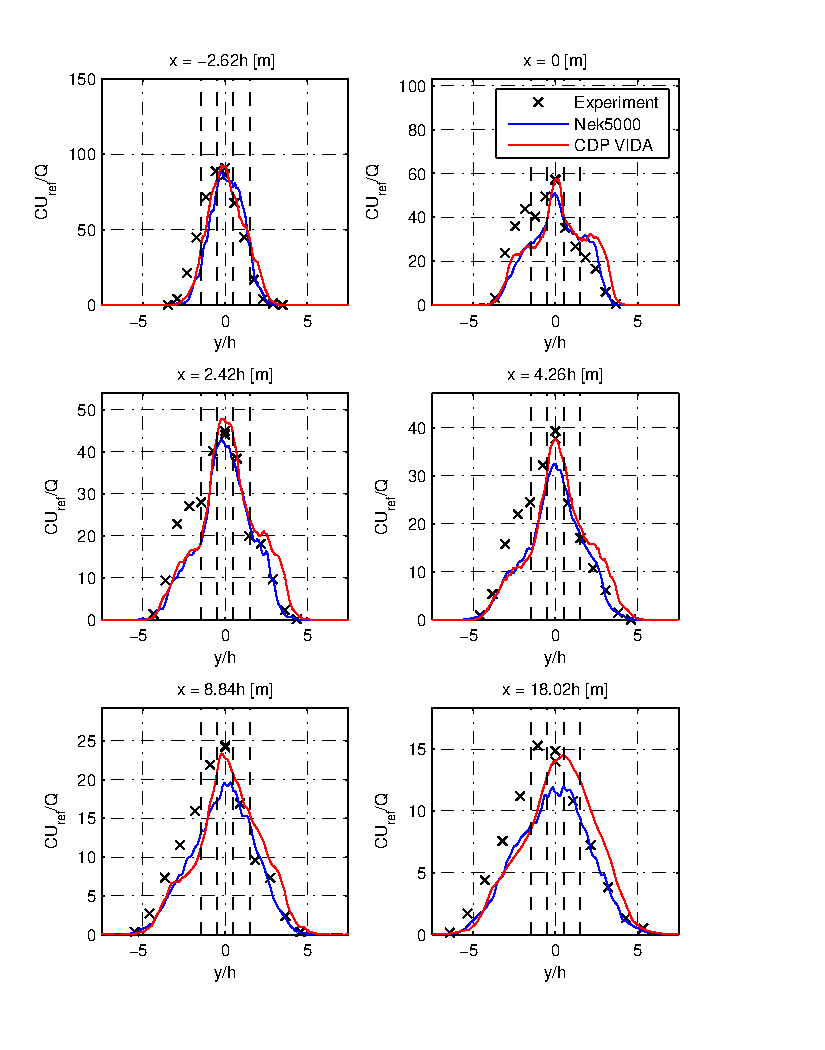
\includegraphics[width=0.8\textwidth]{Figures/NekcH.pdf}
	\caption{Time-averaged concentration with a sample time of $18.00$ s at $z/H = 0.025$ plotted horizontally and scaled 
	with the free-stream velocity and emission rate. Compared against wind tunnel data.
Two dashed lines on either side of the centerline represent the canyon.}
	\label{fig:cHfilter}
\end{figure}
%
Discuss the plot... 


\colorbox{green}{redo these simulation in case they were started to early.}
%
\begin{figure}[h]
	\centering
	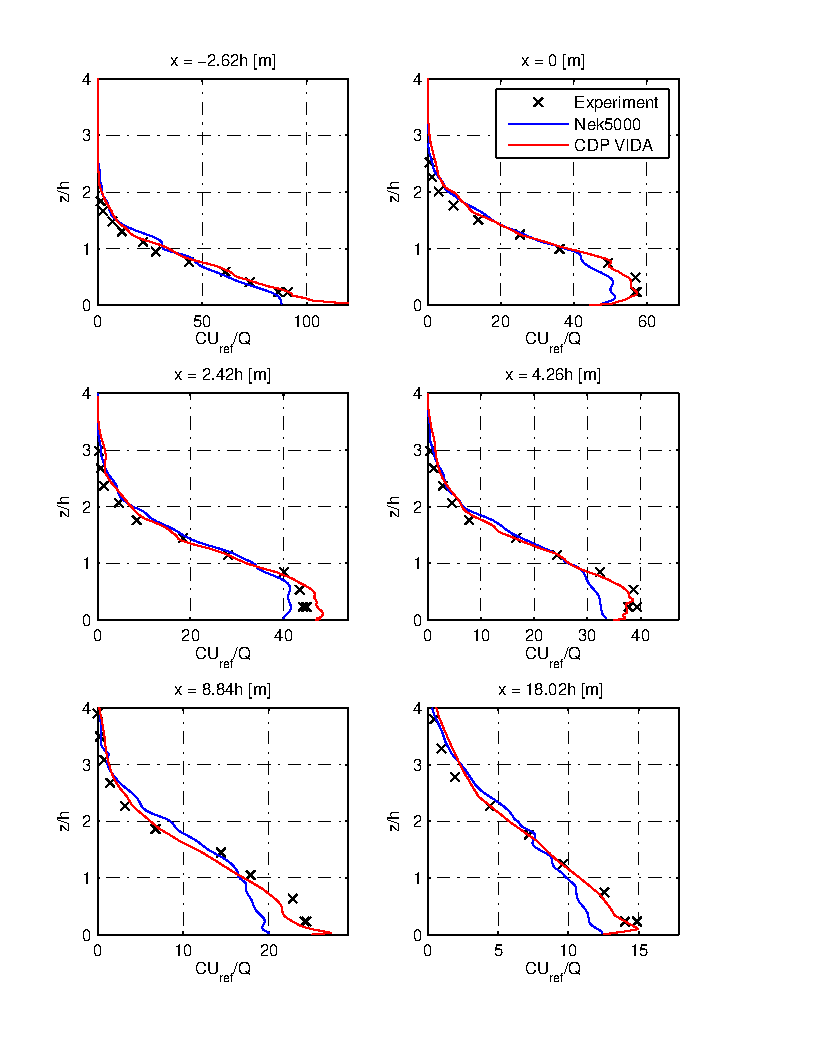
\includegraphics[width=0.8\textwidth]{Figures/NekcV.pdf}
	\caption{Time-averaged concentration with a sample time of $18.00$ s at $y = 0$ plotted
    vertically and scaled 
	with the free-stream velocity and emission rate. Compared against wind tunnel data.
Two dashed lines on either side of the centerline represent the canyon.}
	\label{fig:cVfilter}
\end{figure}
%

\subsection{Dynamic Smagorinsky}
Applying a subgrid scale model to the problem should imply a more accurate result 
since the grid is not sufficiently fine to resolve the finest eddies. 
%
\begin{figure}[h]
	\centering
	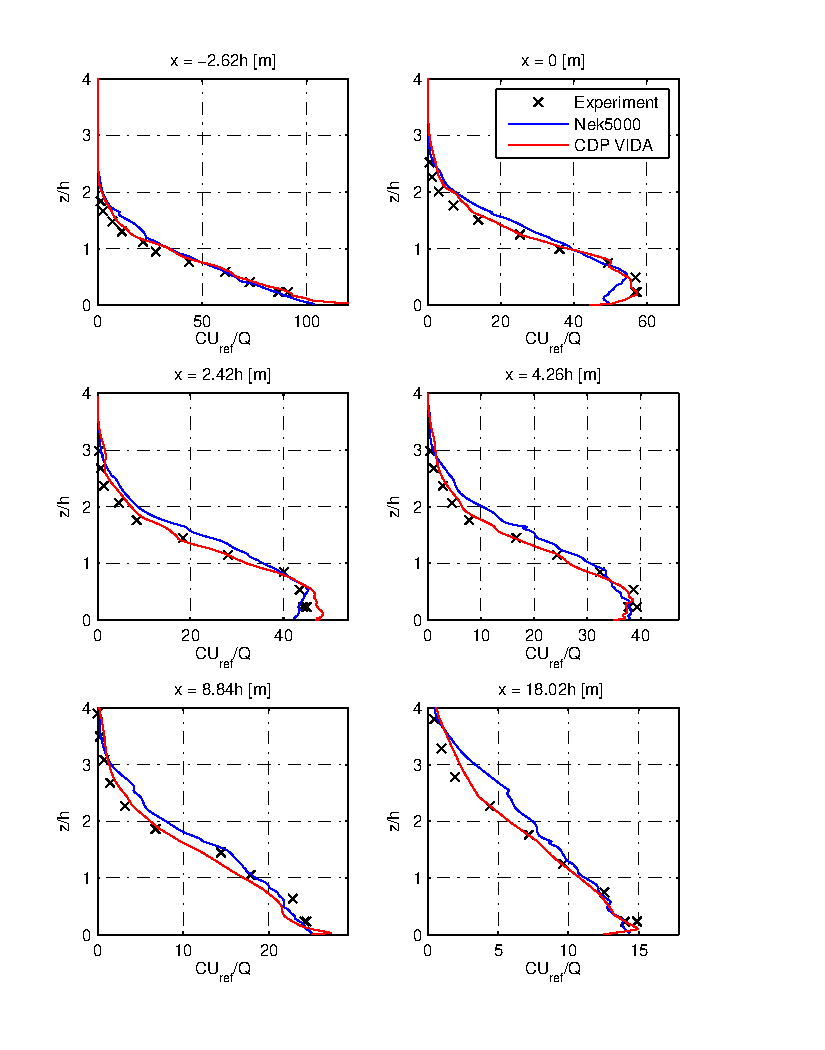
\includegraphics[width=0.8\textwidth]{Figures/Nek_smag_cV.pdf}
	\caption{Time-averaged concentration with a sample time of $22.00$ s at $y = 0$ plotted
    vertically and scaled 
	with the free-stream velocity and emission rate. Compared against wind tunnel data.
Two dashed lines on either side of the centerline represent the canyon.}
	\label{fig:cVsmag}
\end{figure}
%
%
\begin{figure}[h]
	\centering
	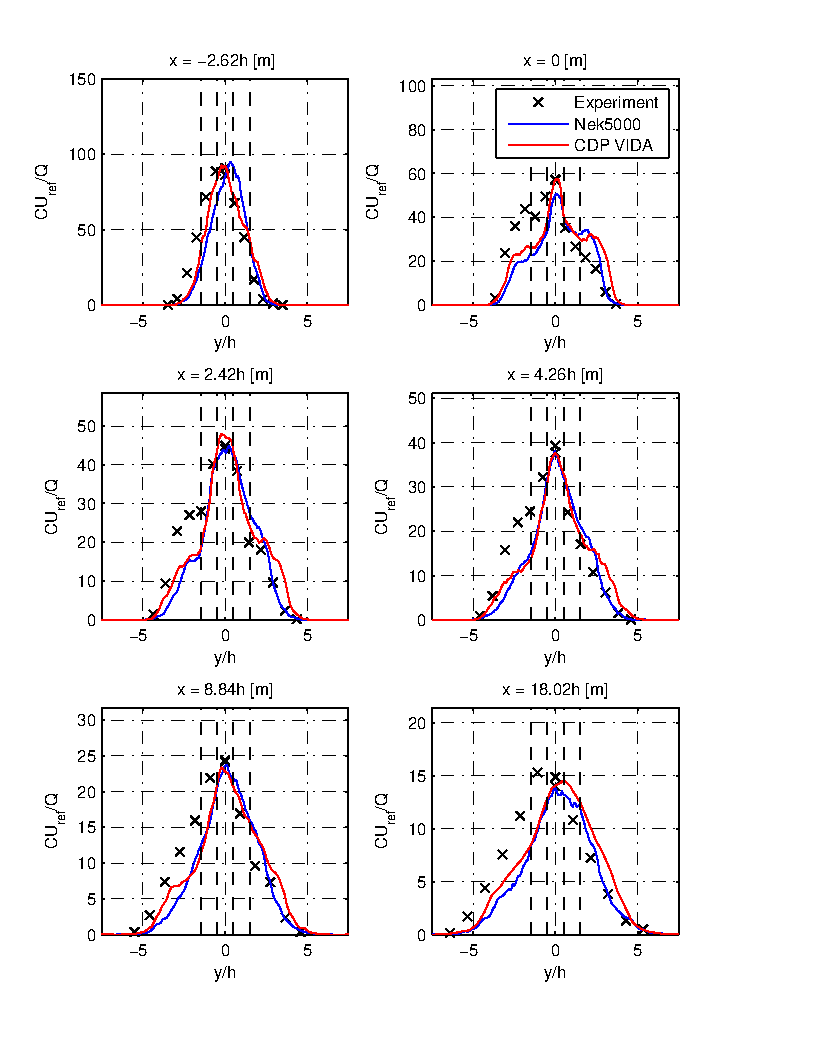
\includegraphics[width=0.8\textwidth]{Figures/Nek_smag_cH.pdf}
	\caption{Time-averaged concentration with a sample time of $22.00$ s at $y = 0$ plotted
    vertically and scaled 
	with the free-stream velocity and emission rate. Compared against wind tunnel data.
Two dashed lines on either side of the centerline represent the canyon.}
	\label{fig:cVsmag}
\end{figure}
%
%
\begin{figure}[h]
	\centering
	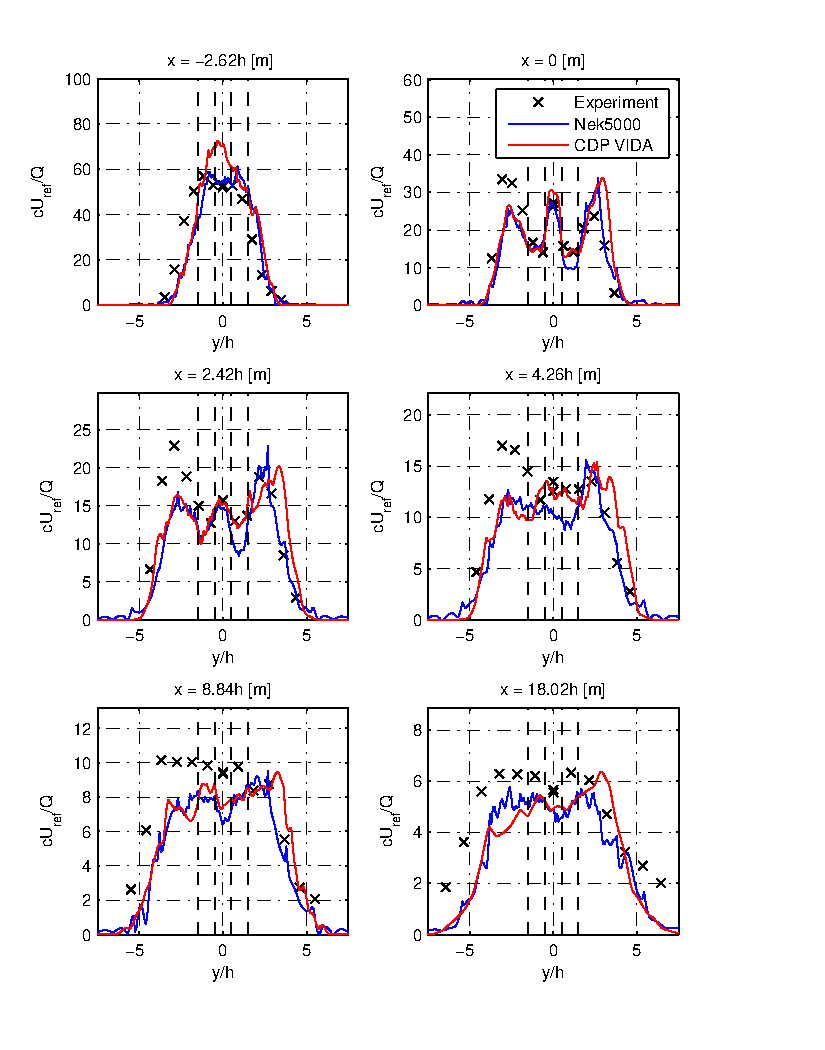
\includegraphics[width=0.8\textwidth]{Figures/Nek_smag_cfluctH.pdf}
	\caption{Time-averaged concentration with a sample time of $22.00$ s at $y = 0$ plotted
    vertically and scaled 
	with the free-stream velocity and emission rate. Compared against wind tunnel data.
Two dashed lines on either side of the centerline represent the canyon.}
	\label{fig:cVsmag}
\end{figure}
%

\section{Discussion and Conclusion}
\colorbox{green}{How did Nek perform overall, user-friendly ?,correctness,speed etc.}

